\documentclass{ctexart}
\usepackage{tabularx}
\usepackage{amssymb}
\usepackage{amsmath}
\usepackage{graphicx}
\author{JohnsonLee}
\title{重积分}
\date{\today}

\begin{document}
  \begin{titlepage}
    \maketitle
    \tableofcontents
  \end{titlepage}
  \section{二重积分的概念与性质}
  \subsection{定义}
    四步走: 分割 $\rightarrow$ 近似 $\rightarrow$求和$\rightarrow$取极限

    一重定积分的定义我们要解决两个问题:\subparagraph{1} 面积的定义\subparagraph{2} 找出计算面积的方法

    一重定积分解决面积问题,二重积分解决体积问题

    \paragraph{1.体积问题}
      \subparagraph{曲顶柱体}
      以$xoy$面上的闭区域$D$为底,侧面以$D$的边界曲线为准县而母线平行于$z$轴的柱面,顶是曲面$z = f(x,y)$,(和一重积分以函数为边界类比),$f(x,y) \ge 0$且在$D$上连续
      \begin{figure}[htbp]
        \centering
        \caption{二重积分定义示意图}
        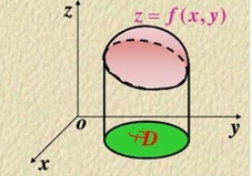
\includegraphics[width = 7cm]{PictrueNote/Volume.png}
      \end{figure}
    四步走: 分割 $\rightarrow$ 近似 $\rightarrow$求和$\rightarrow$取极限
    区域$D$分成一小圈一小圈,近似成柱体,再把柱体加起来,令最大的圈半径都趋近0,就可以了\quad
      \begin{figure}[htb]
        \centering
        \caption{二重积分计算法示意图}
        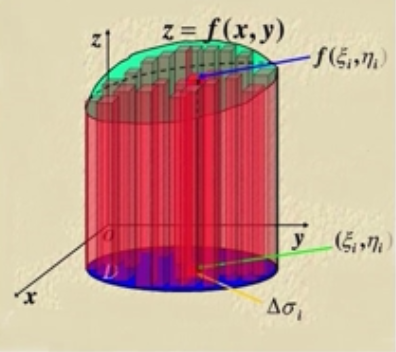
\includegraphics[width = 7cm]{PictrueNote/Howtosum.png}
      \end{figure}

      \paragraph{求非均匀平面薄片的质量}
      \begin{figure}[htb]
        \centering
        \caption{非均匀平面薄片的质量算法}
        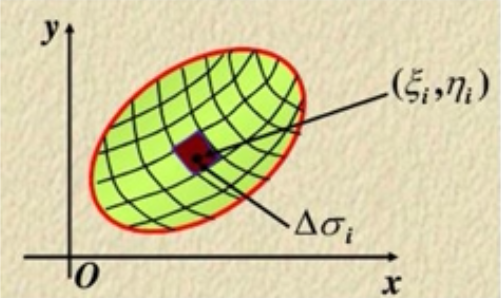
\includegraphics[width = 7cm]{PictrueNote/M.png}
      \end{figure}
        设有一平面薄片,占有$xoy$面上的闭区域$D$,在点$(x,y)$处的面密度为$\mu (x,y)$,假定$\mu(x,y)$在$D$上连续,求平面薄片的质量$M$
          \subparagraph{1.}将薄片分割成n个小块,任取小块$\Delta \sigma_i$近似看作均匀薄片
          \subparagraph{2.}$\Delta M_i \approx \mu(\eta_i,\xi_i )\Delta \sigma_i$
          \subparagraph{3.}$\Delta M \approx  \sum_{i=1}^{n}\mu(\eta_i,\xi_i )\Delta \sigma_i$
          \subparagraph{4.}$\Delta M =  \lim_{\lambda \to 0}\sum_{i=1}^{n}\mu(\eta_i,\xi_i )\Delta \sigma_i$
  \subsection{二重积分的存在定理}
  $f(x,y)$是闭区域长的连续或分片连续函数是则积分存在\footnote{我们直接认为连续函数可积}
  \section{二重积分的计算法}
  \section{二重积分的应用}
  \section{三重积分的概念及其计算法}
  \section{利用柱面坐标和球面坐标计算三重积分}
\end{document}